\chapter{Mikrogesten}

Die grundsätzliche Idee zur Handschrifterkennung ist die Unterteilung der Schrift in sogenannte Mikrogesten. Eine Mikrogeste ist eine simple Bewegung, die beim Schreiben ausgeführt wird. Jeder Buchstabe soll dann aus solchen Mikrogesten aufgebaut werden können. 
Es ist nun natürlich möglich diese Mikrogesten auf beliebige Art zu definieren. Die Hauptkriterien sind, dass die Gesten so einfach wie möglich sein sollen (Für eine optimale Erkennung) und sich untereinander möglichst stark unterscheiden. Je weniger solche Gesten man braucht, desto besser. Man kann jedoch nicht beliebig grobe Gesten wählen, da immer noch alle möglichen Zeichen einzigartig aus solchen Gesten zusammen gebaut werden müssen.

\begin{figure}[h!]
  \centering
    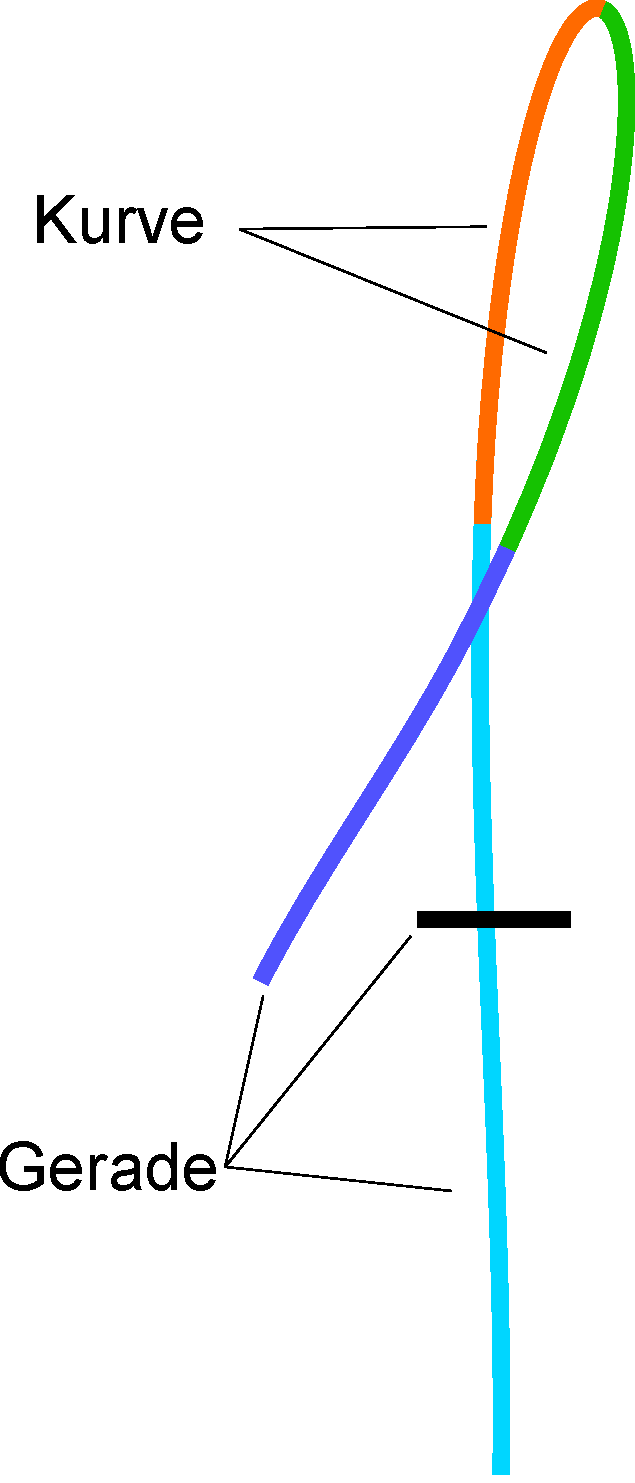
\includegraphics[width=0.2\textwidth]{./img/mikrogesten_beispiel.pdf}
  \caption{Beispiel für die Auftrennung des Buchstaben 'f' in Mikrogesten.}
  \label{mikrogeste_beispiel}
\end{figure}

In der Abbildung \ref{mikrogeste_beispiel} sieht man eine mögliche Aufteilung des Buchstaben 'f' in die Mikrogesten \emph{Kurve} und \emph{Gerade}. Der Buchstabe wird also durch die Abfolge Gerade-Kurve-Kurve-Gerade-Gerade definiert. Nur zwei Mikrogesten sind allerdings zu wenige um alle Zeichen eindeutig abzubilden.

\section{Eigenschaften}
Die Mikrogesten müssen genau definiert werden und können mehr als eine Eigenschaft besitzen:

\subsubsection{Form}
Es ist naheliegend die Mikrogesten hauptsächlich anhand ihrer Form zu unterscheiden. Diese Eigenschaft reicht jedoch nicht, um alle Buchstaben einzigartig zu beschreiben. Zum Beispiel könnte ein 'b' und ein 'p' beides als Gerade-Kreis beschrieben werden. 

\subsubsection{Ausrichtung}
Die Ausrichtung kann auch eine wichtige Eigenschaft sein, z.B. um Querstriche von Längsstrichen zu unterscheiden. Es bietet sich an, die Mikrogesten in eine diskrete Anzahl Richtungen abzubilden, um später die Erkennung im Graph zu vereinfachen.

\subsubsection{Länge}
Für Geraden kann die Länge eine wichtige Rolle spielen: Zum Beispiel ist der Unterschied zwischen 'q' und 'a' nur die Länge der Geraden.  Die Länge wird normalerweise nach dem Liniensystem der Schrift definiert (siehe Abbildung \ref{liniensystem}). Es wird unterschieden zwischen Linien die nur Mittellänge haben und solchen die Ober- oder Unterlänge haben.

\subsubsection{Position}
Die Schrift kann in drei Bereiche Unterteilt werden: Mittel-, Unter- und Oberlänge \cite{typo_linien}. Die Mikrogesten können sich generell in einem oder zwei dieser Bereiche befinden. Dies kann in spezialfällen die Unterscheidung ermöglichen: Zum Beispiel Besitzen 'p' und 'b' den gleichen Aufbau, jedoch befindet sich die Gerade an einer anderen Position.

\begin{figure}[h!]
  \centering
    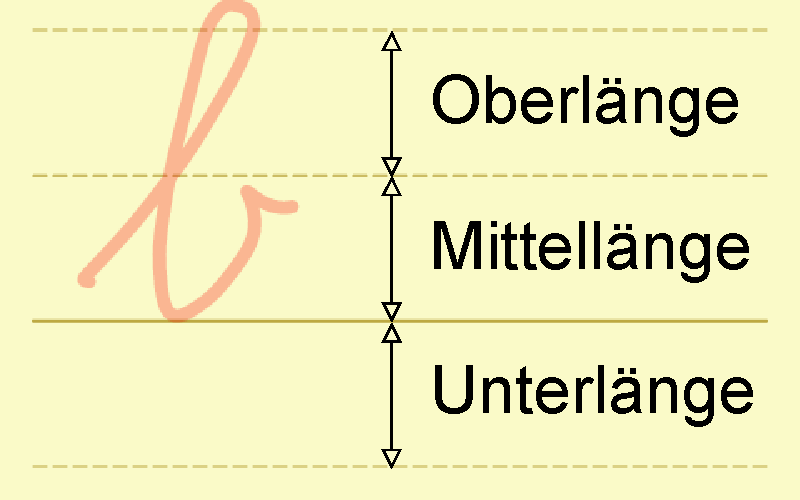
\includegraphics[width=0.4\textwidth]{./img/liniensystem.pdf}
  \caption{Unterteilung der Buchstaben in Mittel-, Unter- und Oberlänge}
  \label{liniensystem}
\end{figure}

\section{Typen}
\subsection{Variante A}
Variante A der Mikrogesten haben wir aus der bestehenden Projektarbeit \cite{zeichenerkennung_pa} zu diesem Thema übernommen: 

Es sind folgende Mikrogesten definiert:
\begin{itemize}
\item Gerade
\item Spitzkehre
\item Schwache Krümmung
\item Starke Krümmung
\end{itemize}

Es wird ausserdem noch berücksichtigt, ob der erkannte Buchstabe Ober- oder Unterlänge hat, um ähnliche Buchstaben zu unterscheiden. Richtung und Position der Mikrogesten werden nicht berücksichtigt.

\subsection{Variante B}
Variante B wurde von uns selbst erarbeitet, um eine bessere Toleranz gegenüber unterschiedlichen Schreibstilen zu erhalten:\begin{itemize}
\item Kreis
\item Halbkreis
\item Lange Gerade
\item Kurze Gerade
\end{itemize}

Die Bezeichnungen Kreis und Halbkreis könnten etwas irreführend sein: Die Pfade müssen nicht genau kreisförmig sein, sondern jeder geschlossene Pfad gilt als Kreis und jeder gebogene Pfad gilt als Halbkreis. Es wird zusätzlich noch die Position und Richtung der Mikrogesten berücksichtigt. Die daraus resultierenden Kombinationen sind in Tabelle \ref{varb_directions} ersichtlich.

\begin{table}[h!]
  \begin{center}
\[
    \begin{array}{l | c | c }
    Richtung & Halbkreis & Gerade \\
    \hline
   \mbox{Vertikal} & \subset & | \\
    \mbox{Vorwärts} & \cap & \backslash \\
    \mbox{Horizontal} & \supset & - \\
    \mbox{Rückwärts} & \cup & / \\
    \hline
    \end{array}
\]
  \end{center}
  \caption{Die vier Richtungen für Halbkreis und Gerade}
  \label{varb_directions}
\end{table}


\section{Abbildung von Zeichen}
Jedes Zeichen muss nun mit den vorgegebenen Mikrogesten aufgebaut werden. Abbildung \ref{beispiel_aufbau} zeigt wie dies theoretisch mit Variante A und B aussieht. Dieses Beispiel berücksichtigt nur Blockschrift. Für die Kursivschrift ist ein anderer Aufbau nötig. Dort kommt die Position der Mikrogesten zum Zuge: Einige Kursivbuchstaben haben zum Beispiel einen Kreis im Oberlängen- oder Unterlängen-Bereich.

Eine weitere Besonderheit der Kursivschrift ist das zusammenhängen von Buchstaben. Dieses Problem kann mit Hilfe von Postfix-Mikrogesten gelöst werden. Damit ist lediglich eine oder mehrere optionale Mikrogesten gemeint, die am Ende der Mikrogesten-Folge angehängt sind. Es müssen mehrere Verbindungsgesten möglich sein, da diese je nach verbundenen Buchstaben anders ist.

Für die Variante A wurden von der vorhergehenden Projektgruppe Präfixe verwendet, um die Buchstabenverbindung zu gewährleisten.

Folglich gibt es für jeden Buchstaben zwei Möglichkeiten, geschrieben zu werden und bei der Kursiv-Variante gibt es noch optionale Zeichen-Teile. 

\begin{table}[h!]
  \begin{center}
\[
    \begin{array}{l | c | c }
    Buchstabe & \mbox{\emph{Aufbau Variante A}} & \mbox{\emph{Aufbau Variante B}} \\
   \hline\noalign{\smallskip}
   \mbox{a} & 
	 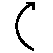
\includegraphics[width=15pt]{./img/a_schwach_uhrzeiger.pdf}   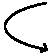
\includegraphics[width=15pt]{./img/a_stark_gegenuhrzeiger.pdf}    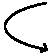
\includegraphics[width=15pt]{./img/a_stark_gegenuhrzeiger.pdf}   & 
	\bigcirc \; | \\
   \hline\noalign{\smallskip}

    \mbox{b} & 
		 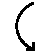
\includegraphics[width=15pt]{./img/a_schwach_gegenuhrzeiger.pdf}  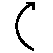
\includegraphics[width=15pt]{./img/a_schwach_uhrzeiger.pdf}   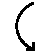
\includegraphics[width=15pt]{./img/a_schwach_gegenuhrzeiger.pdf}   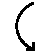
\includegraphics[width=15pt]{./img/a_schwach_gegenuhrzeiger.pdf} & 
		 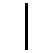
\includegraphics[width=15pt]{./img/a_gerade.pdf} \; \bigcirc \\ 
  \hline\noalign{\smallskip}

    \mbox{c} &
		 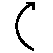
\includegraphics[width=15pt]{./img/a_schwach_uhrzeiger.pdf}   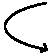
\includegraphics[width=15pt]{./img/a_stark_gegenuhrzeiger.pdf}  & 
		\subset \\ 
  \hline\noalign{\smallskip}

    \mbox{d} & 
		 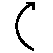
\includegraphics[width=15pt]{./img/a_schwach_uhrzeiger.pdf}   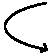
\includegraphics[width=15pt]{./img/a_stark_gegenuhrzeiger.pdf}   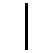
\includegraphics[width=15pt]{./img/a_gerade.pdf}   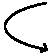
\includegraphics[width=15pt]{./img/a_stark_gegenuhrzeiger.pdf}  & 
		\bigcirc 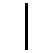
\includegraphics[width=15pt]{./img/a_gerade.pdf} \\
   \hline
    \end{array}
\]
  \end{center}
  \caption{Beispiel-Aufbau der Buchstaben a, b c und d}
  \label{beispiel_aufbau}
\end{table}

Im Anhang befindet sich eine Tabelle mit dem Aufbau aller Buchstaben.

\chapter{Graph}
Nachdem man nun die Buchstaben in Mikrogesten aufgeteilt hat, muss man noch herausfinden, welche Folge von Mikrogesten welchen Buchstaben darstellt. Eine Möglichkeit dies zu tun ist die Verwendung eines zyklischen gerichteten Graphen \cite{diestel2006graphentheorie}. Wie im vorherigen Kapitel beschrieben, werden alle Buchstaben durch Mikrogesten-Folgen beschrieben. Jede Mikrogeste der Folge wird im Graph als Knoten dargestellt. Mit einer intelligenten Verknüpfung der Knoten lassen sich so beliebige Abweichungen und auch mehrere Buchstaben abbilden. 

Die Erkennung funktioniert im Prinzip so, dass die Liste der erkannten Mikrogesten der Fahrplan für den Graph darstellt. Ausgehend von einem Startknoten wird immer die nächste Mikrogeste aus der Liste entnommen und auf den passenden Knoten gewechselt. Nachdem alle Mikrogesten so abgearbeitet wurden, sollte man auf einem Knoten mit einem zugehörigen Buchstaben gelandet sein.

In Abbildung \ref{beispiel_graph} sieht man einen ganz simplen solchen Graphen. 

\begin{figure}[h!]
  \centering
    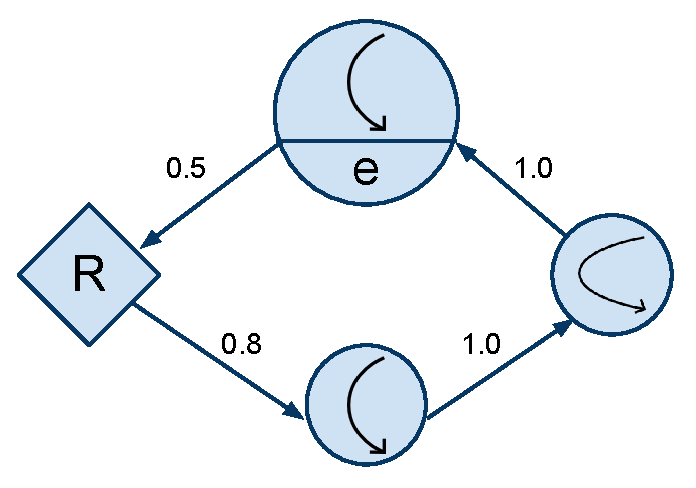
\includegraphics[width=0.5\textwidth]{./img/BeispielGraph.pdf}
  \caption{Ein sehr einfacher Graph für die Erkennung des Buchstaben 'e'}
  \label{beispiel_graph}
\end{figure}

\section{Aufbau}
Der Graph besitzt einen Eintrittspunkt, den \emph{Root-Node}. Von diesem aus wird jeweils die Buchstaben-Erkennung gestartet. Jedes Mal wenn der Pfad auf dem Graph wieder zurück auf den Root-Node führt, bedeutet dies dass die Buchstaben-Erkennung abgeschlossen ist und ein neuer Buchstaben beginnt. 

Die restlichen Nodes beinhalten alle eine bestimmte Mikrogeste und optional ein Zeichen. Die Kanten sind alle gewichtet, um einen Pfad durch den Graphen zu bewerten. Es ist möglich, dass mit einer bestimmten Menge Mikrogesten der Graph auf mehrere Arten beschritten werden kann. Um diese verschiedenen Pfade zu vergleichen wird die Gewichtung der beschrittenen Kanten verglichen.

\section{Erkennungswahrscheinlichkeit}
Jeder Node besitzt eine bestimmte Wahrscheinlichkeit. Beim durchlaufen des Pfades werden alle Wahrscheinlichkeiten multipliziert. So können häufige Mikrogesten-Abfolgen gestärkt werden und seltene geschwächt. Die resultierende Pfadwahrscheinlichkeit hilft, die beste Lösung auszuwählen.

\section{Erkennung von Zeichen}

In Abbildung \ref{beispiel_graph_ablauf} ist aufgezeigt, wie der Graph entsprechend der erkannten Mikrogesten abgeschritten wird. Was allerdings im Beispiel nicht berücksichtigt ist: Es ist sehr wahrscheinlich, dass mehr als eine mögliche Lösung existiert. Bei mehreren Lösungen muss bestimmt werden, welche Lösung am besten ist. 

\begin{figure}[h!]
  \centering
    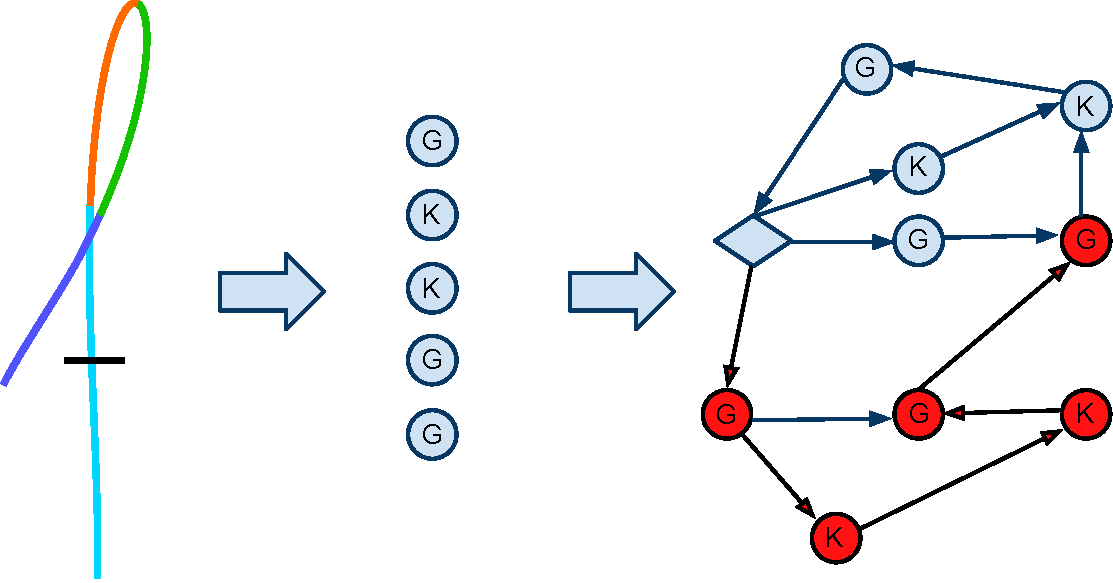
\includegraphics[width=\textwidth]{./img/graph_ablauf_beispiel.pdf}
  \caption{Beispiel des Ablaufs Eingabe - Mikrogesten-Erkennung - Buchstaben-Erkennung}
  \label{beispiel_graph_ablauf}
\end{figure}
